\section{Existing vertical jump calculators}
There are few \textit{modern} jump calculators on the market right now. None are combined with existing fitness platforms -
our research shows all of them being standalone mobile or web applications (\labelcref{research:fitness-meter,research:whats-my-vert,research:my-jump}).
\par
There are multiple methods of measuring jump height, often this is important to athletes 
where success is caused/correlated with jump ability i.e. Sprinting \cite{jump-sprint-link}, American football, Basketball, Volleyball.
We also know vertical jump is an important test to assess the explosive strength of the leg
musculature of athletes \cite{aspects-of-strength,nsa-strength-in-athletes}.
We'll be using the time-in-air (TIA) to estimate jump height. Whilst this is inevitably not perfectly
accurate, when using a force plate \footnote{A measuring instrument that measures the ground reaction forces generated by somebody.}
it is no worse than other methods (in terms of consistency) \cite{measuring-jump-paper}.
Thereby still proving useful to the target demographic.
\par
To summarise, the vertical jump calculator created for the project is intended for use as a measurement of progress
and not a concrete result. There will be some deviation from other measurements (such as using a \href{https://www.topendsports.com/testing/products/vertical-jump/vertec.htm}{Vertec}).
\pagebreak 

\subsection{Maths behind calculating vertical jump using video}
\label{research:jump-maths}
Below we'll be considering the physics \cite{hoopsgeek-maths} involved in finding vertical jump height using
\textbf{only smartphone video footage}.
\par
To explain the forces demonstrated in a countermovement jump (CMJ)\footnote{A vertical jump test performed by having an athlete quickly squat to a self-selected depth and then jump as high as possible.}
we'll be considering the 5 phases of action involved (\cref{fig:jump-phases}).
\begin{figure}[H]
	\centering
	\begin{minipage}[c]{0.5\textwidth}
		\caption{Motion phase of countermovement jump (CMJ). 1: Rest. Before jump. \linebreak2: Countermovement. 3: Push to ground. \linebreak4: Jump. Fly. 1 * : Rest. Land. \linebreak Vertical position of torso is y position \cite{jumping-phases-picture}.}
		\label{fig:jump-phases}
	\end{minipage}%
	\begin{minipage}[c]{0.5\textwidth}
		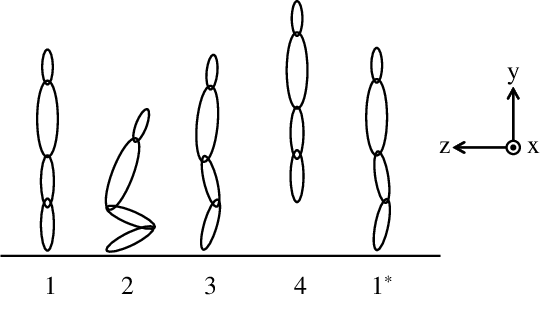
\includegraphics[width=\textwidth]{jump-maths/phases-of-cmj.png}
	\end{minipage}
\end{figure}
\vspace*{-5mm}
\begin{figure}[H]
	\centering
	\resizebox{0.7\linewidth}{!}{
    \noindent
    \begin{tikzpicture}[trim left=0cm]
        \centering
        \begin{axis}[
                axis on top,
                axis lines = left,
                xlabel = {time in seconds (s)},
                ylabel = {Force in Newtons},
                xmin=-1, xmax=1,
                ymin=0, ymax=2600,
                xtick={-1.0,-0.5,0.0,0.5,1.0},
                ytick={500,1000,1500,2000},
                axis line style={opaque},
                label style={font=\tiny},
                ticklabel style={font=\tiny},
                tick style={draw=none},
                legend style={draw=none},
            ]

            % Define axis lines
            % Gravity line defined
            \path [
                name path=axis,
            ]
            (axis cs:-1,0) -- (axis cs:1,0);


            % Gravity line defined
            \addplot [
                name path=gravity,
                color=gray,
                fill=gray!10!,
                draw=none,
                area legend,
            ]
            {1000};

            %Below the main force of jumper is defined
            \addplot [
                name path=A,
                domain=-1:1,
                samples=11,
                color=red,
                smooth,
                line width=1pt,
                tension={0.15}
            ]
            coordinates {
                    (-1,1000)(-0.6,1000)(-0.5,500)(-0.4,1000)(-0.3,1500)(-0.2,2000)(0.0,0.0)(0.5,0.0)(0.6,2100)(0.7,1250)(0.8,1600)(0.9,1000)(1,1000)
                };

            \addplot [
                name path=phase2end,
                domain=-0.6:-0.4,
                samples=11,
                opacity=0,
            ]
            coordinates {
                    (-0.4,1000)(-0.35,1250)(-0.205,2000)(0.0,0.0)(0.5,0.0)(0.6,2100)(0.7,1250)(0.8,1600)(0.9,1000)(1,1000)
                };

            \addplot [
                name path=phase3start,
                domain=-0.4:-0.2,
                samples=11,
                opacity=0,
            ]
            coordinates {
                    (-0.25,1000)(-0.25,1750)(-0.205,2000)(0.0,0.0)(0.5,0.0)(0.6,2100)(0.7,1250)(0.8,1600)(0.9,1000)(1,1000)
                };

            \addplot [
                name path=phase4start,
                domain=-0.4:-0.2,
                samples=11,
                opacity=0,
            ]
            coordinates {
                    (-0.1,1000)(0.0,0.0)(0.5,0.0)(0.6,2100)(0.7,1250)(0.8,1600)(0.9,1000)(1,1000)
                };


            \addplot [
                domain=0:0.5,
                samples=11,
                color=red,
                line width=2pt,
            ]
            coordinates {
                    (0,0)(0.5,0)
                };

            % Coloring the phase 1 decline blue
            \addplot [
                fill=blue,
                fill opacity = 0.2,
            ]
            fill between[
                    of=A and phase2end
                ];
            % Coloring the phase 1 incline orange
            \addplot [
                fill=orange,
                fill opacity = 0.2,
            ]
            fill between[
                    of=phase2end and phase3start
                ];
            % Coloring the phase 3 decline orange
            \addplot [
                fill=yellow,
                fill opacity = 0.2,
            ]
            fill between[
                    of=phase3start and phase4start
                ];
            % Coloring final phase
            \addplot [fill=green,fill opacity = 0.2] fill between[
                    of=A and gravity, soft clip={domain=0.55:1}
                ];

            % Coloring the gravity line
            \addplot [gray!10!] fill between[
                    of=A and axis, soft clip={domain=-1:-0.4}
                ];
            \addplot [gray!10!] fill between[
                    of=gravity and axis, soft clip={domain=-0.4:-0.1}
                ];
            \addplot [gray!10!] fill between[
                    of=A and axis, soft clip={domain=-0.1:0.55}
                ];
            \addplot [gray!10!] fill between[
                    of=gravity and axis, soft clip={domain=0.55:1}
                ];

            \legend{
                \tiny Force of Gravity,
                \tiny Force of Jumper Movement,
            }


            % The phase 1 bending label (70Ns)
            \addplot[mark=none, color = blue] coordinates {(-0.475,930)} node[pin=100:{\tiny 70Ns}]{} ;
            % Phase grey marks
            \addplot[mark=*, color=black!80!, draw opacity = 0] coordinates {(-0.6,1000)(-0.4,1000)(-0.26,1750)(0,0)(0.5,0)};
            % The phase 2 label (70Ns)
            \addplot[mark=none, color = orange] coordinates {(-0.31,1250)} node[pin=100:{\tiny 70Ns}]{} ;
            % The phase 3 label (245Ns)
            \addplot[mark=none, color = yellow] coordinates {(-0.16,1250)} node[pin=80:{\tiny 245Ns}]{} ;
            % The phase 4 label (245Ns)
            \addplot[mark=none, color = green] coordinates {(0.600,1250)} node[pin=100:{\tiny 245Ns}]{} ;


        \end{axis}
    \end{tikzpicture}}
	\vspace*{-5mm}
	\caption{Ground reaction forces during vertical jump.}
	\label{fig:jump-phases-graph}
\end{figure}
\pagebreak

We'll be using the above, simplified force plate analysis (\cref{fig:jump-phases-graph}),
to delve further into the phases of a jump and the mathematics. 
In reality the force curve wouldn't be so smooth
but this should demonstrate the phases quite clearly.
\par
\textbf{Phase 1: Rest (Pre-jump)}
\par
Before jumping we can see a flat line at $981$ Newton (\cref{fig:jump-phases-graph}). The athlete isn't jumping, but this is gravity doing it's
work. It's easily explained as $F=m*g$, where $m$ is the mass of the athlete and
$g$ is the acceleration of earth's gravity. $F$ is the force needed to counter the effects of gravity. We know that $g=9.81m/s^2$ on earth, thus:
\[
	\displaystyle
	\begin{aligned}
	981N &= m * 9.81 m/s^2 \\
	=> m &= \frac{981N}{9.81 m/s^2} = 100kg
	\end{aligned}	
\]
Here you can see that the force plate is basically acting as a weighing scale, showing
the force gravity exerts on the athlete.
\par
\textbf{Phase 2: Countermovement}
\par
As seen in \cref{fig:jump-phases}, the countermovement involves
the bending of the knees and typically swinging of the arms to lower the center
of gravity before the jump. The force plate (\cref{fig:jump-phases-graph}) is 
registering forces lower than 981N, which means the athlete is accelerating
in a downward movement.
\par
Recall Newton's 3rd Law of motion; 
which states whenever two objects interact, they exert equal and opposite forces on each other.
Knowing the above, we can define Ground Reaction Force (GRF) as ``the force exerted by the ground
on a body in contact with it''. 
We can describe the forces acting at this time as follows:
\[F_{Jumper} = F_{GRF} - F_{Gravity} \leq0 \]
We can also use the analysis (\cref{fig:jump-phases-graph}) to find
the speed the athlete is moving at before the jump. We know that
$F=ma$ (mass * acceleration), and force is happening over time.
Thus, $Ft=mat$.  
We also know force isn't a constant, it's a function of time and that we can define velocity as $v=at$;
so our formula is:
$$\displaystyle
\int_{t_1}^{t_2} F_{Jumper}(t) \mathrm{d}t = mv$$
where $F_{Jumper}(t)$ is the difference between the GRF and gravity.
\pagebreak
The integral can be calculated from the force plate data. The downward impulse\footnote{Impulse is the integral of a force.} made by
the athlete is shown in the graph (\cref{fig:jump-phases-graph}) as the blue area
below the line representing gravity.
\par
We've assumed the integral (impulse) is -70Ns\footnote{Newton seconds are the units of impulse.}. 
With this, we can conclude that:
\begin{align*}
& \int_{t_1}^{t_2} F(t) \mathrm{d}t = m v \\
&=> -70 N s = 100kg * v \\
&=> v = -70 N s / 100kg = -0.7 m/s
\end{align*}
Therefore, our athlete reaches a peak velocity of -0.7m/s during the countermovement phase.
\par
\textbf{Phase 2.5: Deceleration}
\par
Now we've seen where GRFs are lower than expected due to gravity - we must look for the period
where our athlete has to decelerate the downward movement (pause) before launching up (\cref{fig:jump-phases}).
This should be an equally big impulse to that found above but in the opposite direction.
We can describe this as:
\[\displaystyle \int_{t_2}^{t_3} F_{Jumper}(t) \mathrm{d}t = 70 Ns\]
Because we know $F(t)$ and $t_2$, the algorithm of the force plate analysis
now looks for $t_3$ so the impulse equals 70Ns.
\par
On our graph (\cref{fig:jump-phases-graph}) we have pictured this -
we are looking for the blue and orange areas to be the same size.
\par
\textbf{Phase 3: Push to ground}
\par
The athlete then generates force in preparation for takeoff before the GRFs register as 0
(when they are in flight). They reach some of the peak forces seen.
To assess the velocity during takeoff we use the same technique as Phase 2:
\[
\displaystyle
\int_{t_3}^{t_4} F_{Jumper}(t) \mathrm{d}t = mv	
\]
Pictured in our graph (\cref{fig:jump-phases-graph}) as the yellow area.
\pagebreak

The force plate graph detects 245Ns, so we can determine initial velocity as follows:
\vspace{-3mm}
\begin{align*}
	& 245 N s = 100kg * v \\
	&=> v = 245 N s / 100kg = 2.45 m/s
\end{align*}
\vspace{-5mm}

\textbf{Phase 4: Jump. Flight!}
Here the athlete can't control their velocity any longer; their jump height
is determined by the speed built before and during takeoff. Only gravity is acting on them,
bringing them back to the ground.
\par
We've determined initial velocity was $v(0)=2.45 m/s^2$ and
the gravity of earth has an acceleration of $a=9.81m/s^2$. Plus, the peak
of the jump must have a vertical velocity of zero: $v(t_{peak})=0$.
\par
Using the initial velocity and earths gravity we can find velocity at any given time using:
\vspace{-5mm}
\begin{center}
$
\displaystyle
v(t)=v(0) -a * t
$
\end{center}
\vspace{-5mm}
Thus we can find the velocity at the peak of the jump using:
\[\displaystyle
\begin{aligned}
v(t_{peak}) &= v(0) - a * t_{peak} \\
=> 0 &= v(0) - a * t_{peak} \\
=> t_{peak} &= \frac{v(0)}{a} = \frac{2.45m/s}{9.81m/s^2} = 0.25s
\end{aligned}\]
With the knowledge of $v(t)$ during every moment and knowing the peak of the jump
was 0.25s, we can calculate the jump height as the integral of velocity over the time
it takes to reach the peak of the jump:
\[\displaystyle
\begin{aligned}
h_{jump} &= \int_0^{\frac{v(o)}{a}} \bigg( v(o) - at \bigg) \ \mathrm{d}t= \\
& = v(o)t \ - \ \frac{1}{2} at^2 \ \bigg|_0^{\frac{v(0)}{a}} \\
& = v(0) \left(\frac{v(0)}{a}\right) - \frac{1}{2} a \left(\frac{v(0)}{a}\right)^2 \\
& = \frac{v(0)^2}{a} \ - \ \frac{1}{2} \frac{v(0)^2}{a} \\
=> h_{jump} \ &= \ \frac{1}{2} \frac{v(0)^2}{a} 
\end{aligned}\]
This leaves us with a simple formula for finding jump height
\textit{when we know the initial velocity}. 
For our force plate analysis (\cref{fig:jump-phases-graph}) we get
\[
	\begin{aligned}
		h_{jump} = \frac{1}{2} \frac{(2.45m/s)^2}{9.81 m/s^2} = 0.306m			
	\end{aligned}
\]

Because we only need the initial velocity of an athlete to satisfy our formula,
we don't have to rely on a force plate and expensive equipment.
We simply have to find the initial velocity for a jump that takes 0.5s.
\par
If someone jumps 0.5m high, they must also fall 0.5m after they peak. We have established
velocity is a linear function ($v=at$), thus we can demonstrate the athletes peak
is at the exact middle of the jump. Formally:
\vspace{-3mm}
\[
	\displaystyle
	t_{peak} = 0.5 * t_{hangtime}	
\]
Thus to find the jump height of someone who jumps for 0.5s, we can calculate
the distance of free fall in 0.25s!
\[
	\displaystyle
	\begin{aligned}
	S &= \int_0^{\frac{1}{2} t_{hangtime}} v(t) \; dt \\
	&= \int_0^{\frac{1}{2} t_{hangtime}} a * t \; dt \\
	&= \frac{1}{2} a t^2 \; \bigg|_0^{\frac{1}{2}t_{hangtime}} \\
	&= \frac{1}{2} a \left( \frac{1}{2} t_{hangtime} \right)^2 \\
	&= \frac{1}{8} a \: t_{hangtime}^2 \\
	\end{aligned}	
\]
In the case of a 0.5s hangtime, this gives us (as before with the force plate data):
\[
\begin{aligned}
	S = \frac{1}{8} a \: t_{hangtime}^2 = \frac{1}{8} * 9.81m/s^2 * 0.5^2 = 0.306m
\end{aligned}	
\]
\textbf{\underline{This formula is the crucial component to developing this feature.}} 
We won't be looking
at the physics of ``the landing'' in this document as it is not directly relevant.
However it is worth noting that to counteract the forces created during impact,
the athlete braces themselves and absorbs force - this is notable as the green area
in the graph has a value of 245Ns exactly like the yellow area.
\pagebreak

\subsection{FitnessMeter - Test \& Measure}
\label{research:fitness-meter}
FitnessMeter is an iOS (Apple) exclusive mobile app, used for 
``fitness testing and athletic performance evaluation'' \cite{fitness-meter}.
\begin{figure}[H]
	\centering
	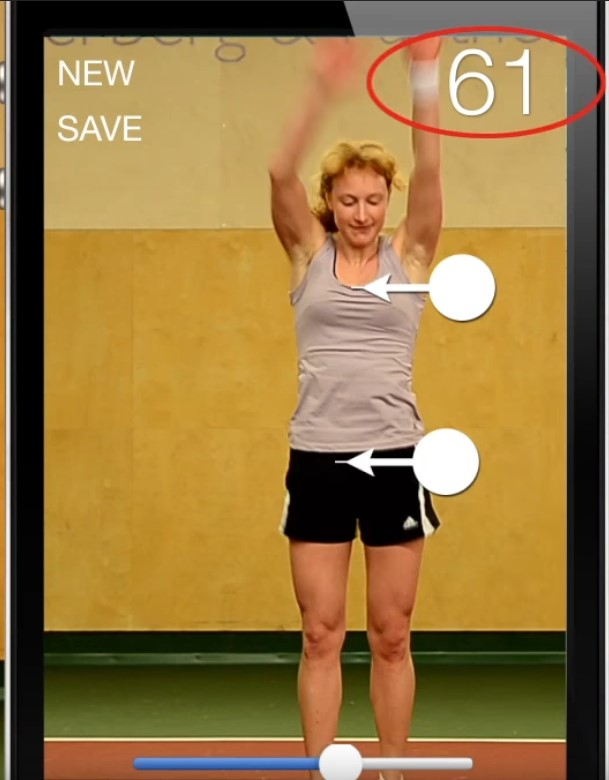
\includegraphics[width=0.2\textwidth]{graphics/fitnessmeter/jumpcalc.jpg}
	\caption{The FitnessMeter vertical jump calculator in use.}
	\label{fig:fitnessmeter-jump}	
\end{figure}
\vspace{-5mm} 
The app uses the change in position of the torso (\cref{fig:fitnessmeter-jump}) to determine jump height. Seemingly by comparing this to their position
in the initial start. Our app aims to comfortably work even when only the feet are in frame. In traditional vertical jump 
tests the athlete maintains straight legs and so the issue of raising the legs/bending the knees to artificially increase
hangtime is not a major concern. \textit{Directions in our app will discourage this technique and establish how to best
find accurate results.}

\subsection{What's My Vertical?}
\label{research:whats-my-vert}
Another iOS only application with poor UI. This application uses the same methods we plan on using; however, the
app serves no purpose beyond the vertical jump measurement and ``dunk calculator'' math.
It lacks further functionality and training support.
\vspace{-5mm}
\begin{figure}[H]
	\centering
	\begin{minipage}{0.45\textwidth}
		\centering
		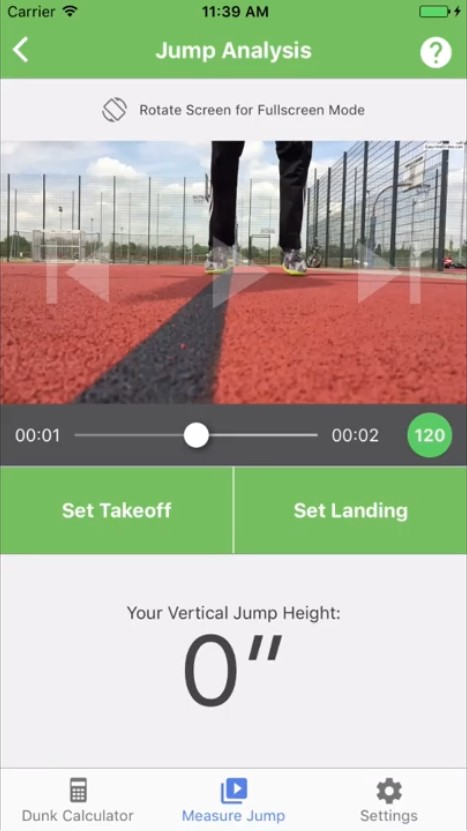
\includegraphics[width=0.4\textwidth]{graphics/whatsmyvert/jumpcalc.jpg}
		\caption{The jump calculator functionality in use.}
		\label{fig:whatsmyvert-jump}
	\end{minipage}%
	\begin{minipage}{0.45\textwidth}
		\centering
		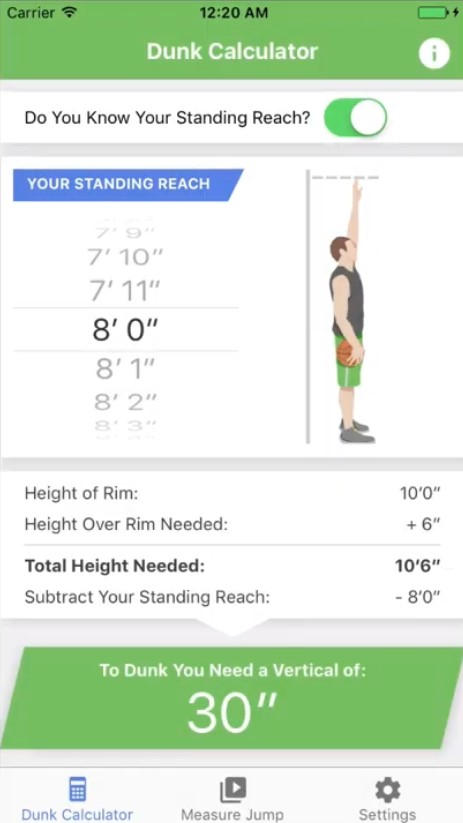
\includegraphics[width=0.4\textwidth]{graphics/whatsmyvert/dunkcalcmaths.jpg}
		\caption{The dunk calculator math being used for estimation.}
		\label{fig:whatsmyvert-math}
	\end{minipage}%
\end{figure}
\pagebreak

As mentioned, we intend on using a very similar system to what's seen here (\cref{fig:whatsmyvert-jump}).
We will consider having a dunk math calculator (\cref{fig:whatsmyvert-math}) as an enhancement and extra feature however this doesn't seem
very useful for our project as the fitness application is not sport specific. Whilst the app will be usable
by basketball players, having basketball specific functionality may limit user growth and alienate
average enthusiasts.

\subsection{My Jump 2}
\label{research:my-jump}
Finally we have looked at ``MyJump 2'' - a cross-platform sports science validated calculator app.
It's been proven to be ``valid, reliable and useful'' \cite{myjump-proof} and provides
the most clarity and insight.
\begin{figure}[H]
	\centering
	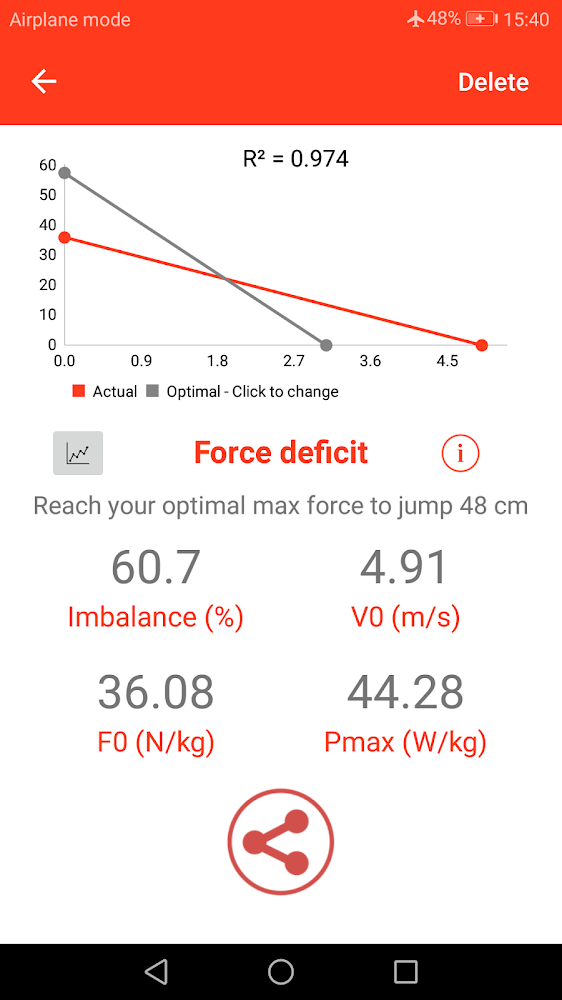
\includegraphics[width=0.2\textwidth]{graphics/myjump2/jump-forces.png}
	\caption{Analysis of a jump and data visualisation provided.}
	\label{fig:myjump2-analysis}	
\end{figure}
The level of precision and insights provided are beyond the scope of our project, as we are focused
on providing consistency first and foremost - thereby allowing our users to track their progress.
This app estimates and visualises forces produced (\cref{fig:myjump2-analysis}), which is useful
in the field of sport science but may not provide sufficient benefit to users for us to dedicate
time to development of a similar feature.